\section{Crossing Fiber Tractography with Uncertainty Reduction}
\label{sec:tracking}
\subsection{Probabilistic Streamline-Based Tractography}
\label{sec:tracking-details}

Our work reduces the data and model uncertainty that affects local fiber directions. Despite this, the fundamental uncertainty that arises from partial volume effects remains, as discussed in Section~\ref{sec:related}: Even if multiple fiber directions were estimated with perfect accuracy, it remains  uncertain which of them should be followed in each step of the tracking. In regions where tracts fan out, there might even be multiple valid ways to continue them. Previous work used deterministic tracking with a branching mechanism to handle these situations \cite{Ankele:CARS2017}. In our work, we follow a probabilistic approach instead. However, its probabilistic nature is limited to deciding which of multiple fiber compartments should be followed next. Unlike most other probabilistic tractography methods \cite{BEHRENS2007144,Jones:2008}, it does not sample a distribution of fiber directions \emph{within} each fiber compartment, since this type of uncertainty is reduced by our bootstrap consensus.

Our tracking acts on multi-vector fields that are pre-computed using any of the methods proposed above. For a given seed point, the streamline is grown iteratively in both directions using Euler
integration\added{, which was sufficient to reconstruct even the curved part of the cingulum bundle at a step size of $0.9\,\mathrm{mm}$}. The multi-vector fields are interpolated to the current position. \added{To keep computational effort manageable, we use trilinear interpolation. It requires solving} another matching problem, since we have to decide which
directions belong together during interpolation. Assuming
smoothness between the voxels, we use the $r$ directions from the last
interpolation step as initial group means $\bar{\mathbf{v}}_i$, $i \in \left\{ 1\dots r 
\right\}$ and assign the vectors from all grid points that are involved in the current interpolation by minimizing the same cost function as in Eq.~(\ref{eq:matching-cost}). \added{If fewer than three vectors are available due to model selection, zero vectors replace the missing ones for the purpose of interpolation.} After all assignments have been made, we \added{re-orient all vectors to have a non-negative dot product with their current group mean,}  compute new group means from them, and iterate the assignment once. To reduce the computational expense, we cache the final assignments, so that they only need to be computed once for each voxel through which we are tracking.

\added{To investigate how this matching step affects the stability of interpolation results, we rotated all vectors at all voxels independently and uniformly at random by up to 10~degrees, and computed the resulting change in tracking direction at 1000 randomly selected streamline vertices, drawn from the experiment in Section~\ref{sec:quantitative-results}. When interpolating the perturbed directions, but keeping the original correspondences, $95\%$ of the deviations were below $5.5^\circ$. Re-matching the perturbed direction increased this only slightly, to $6.3^\circ$. We conclude that ambiguous correspondences contribute relatively little to the overall uncertainty in tracking directions.}

% \begin{figure}
% 	\centering
% 	\begin{subfigure}[b]{0.45\linewidth}
% 		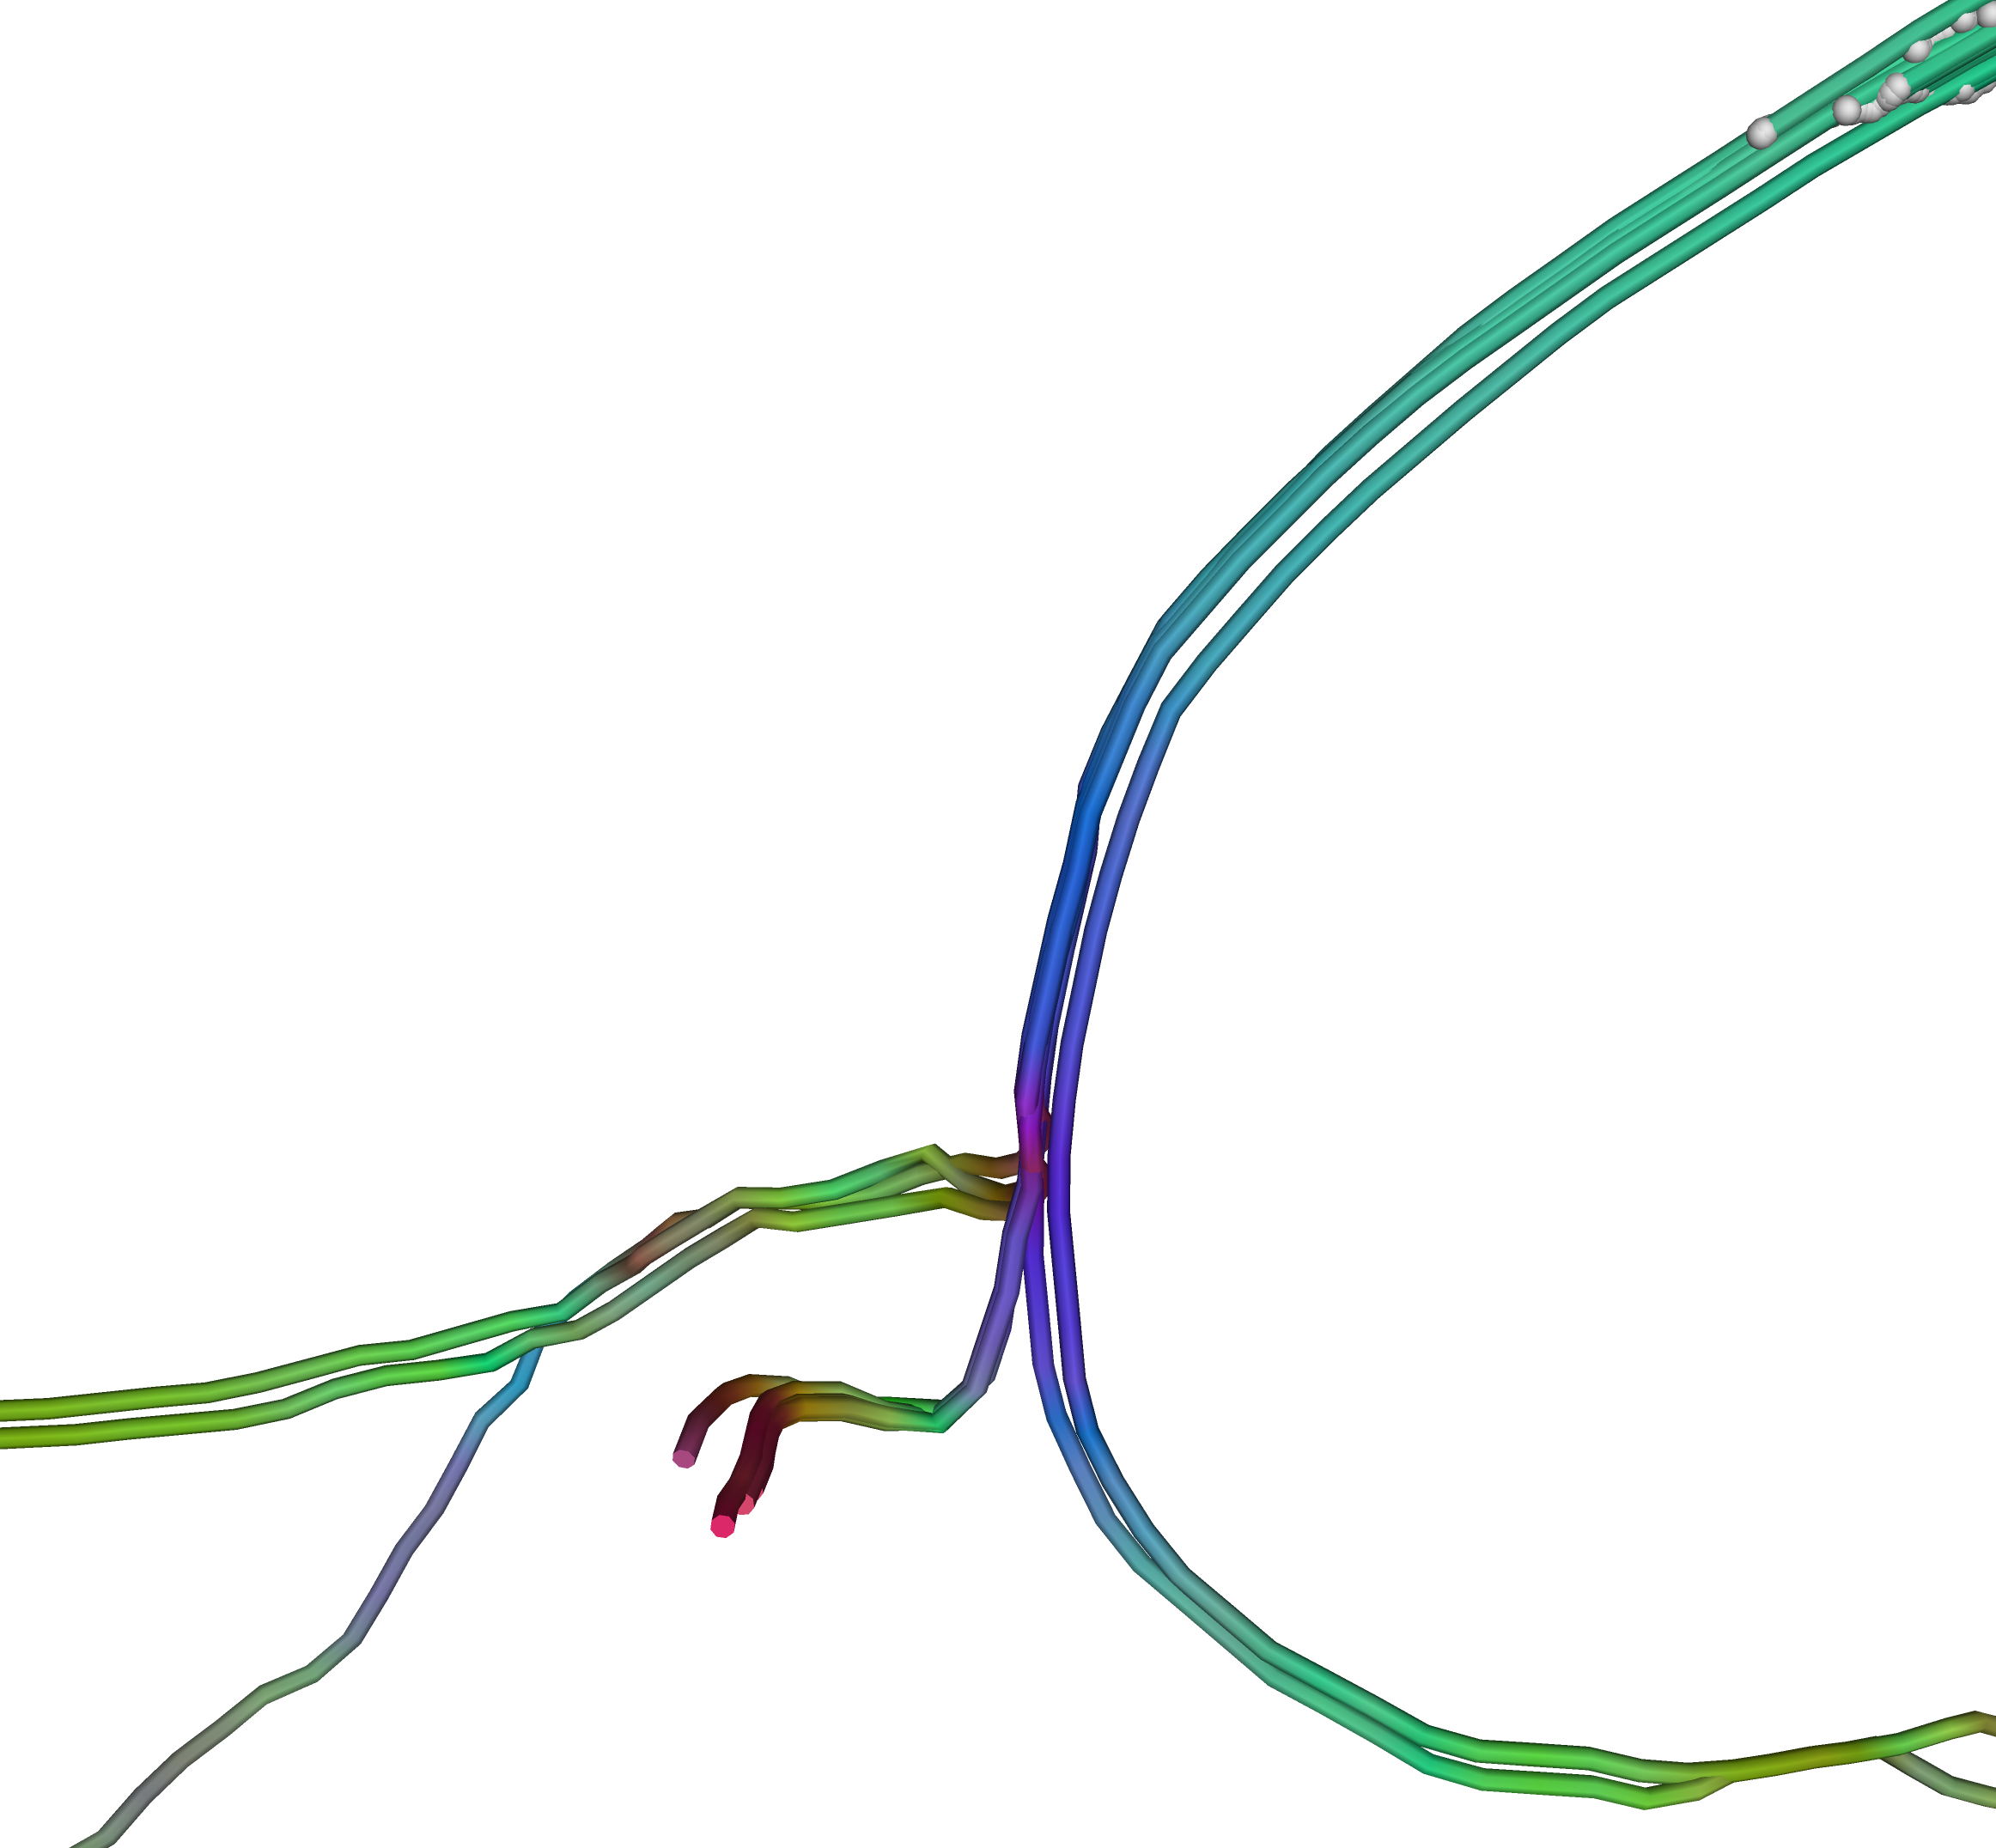
\includegraphics[width=\linewidth]{FACT}
% 		\caption{Nearest neighbor interpolation}
% 	\end{subfigure}
% 	\begin{subfigure}[b]{0.45\linewidth}
% 		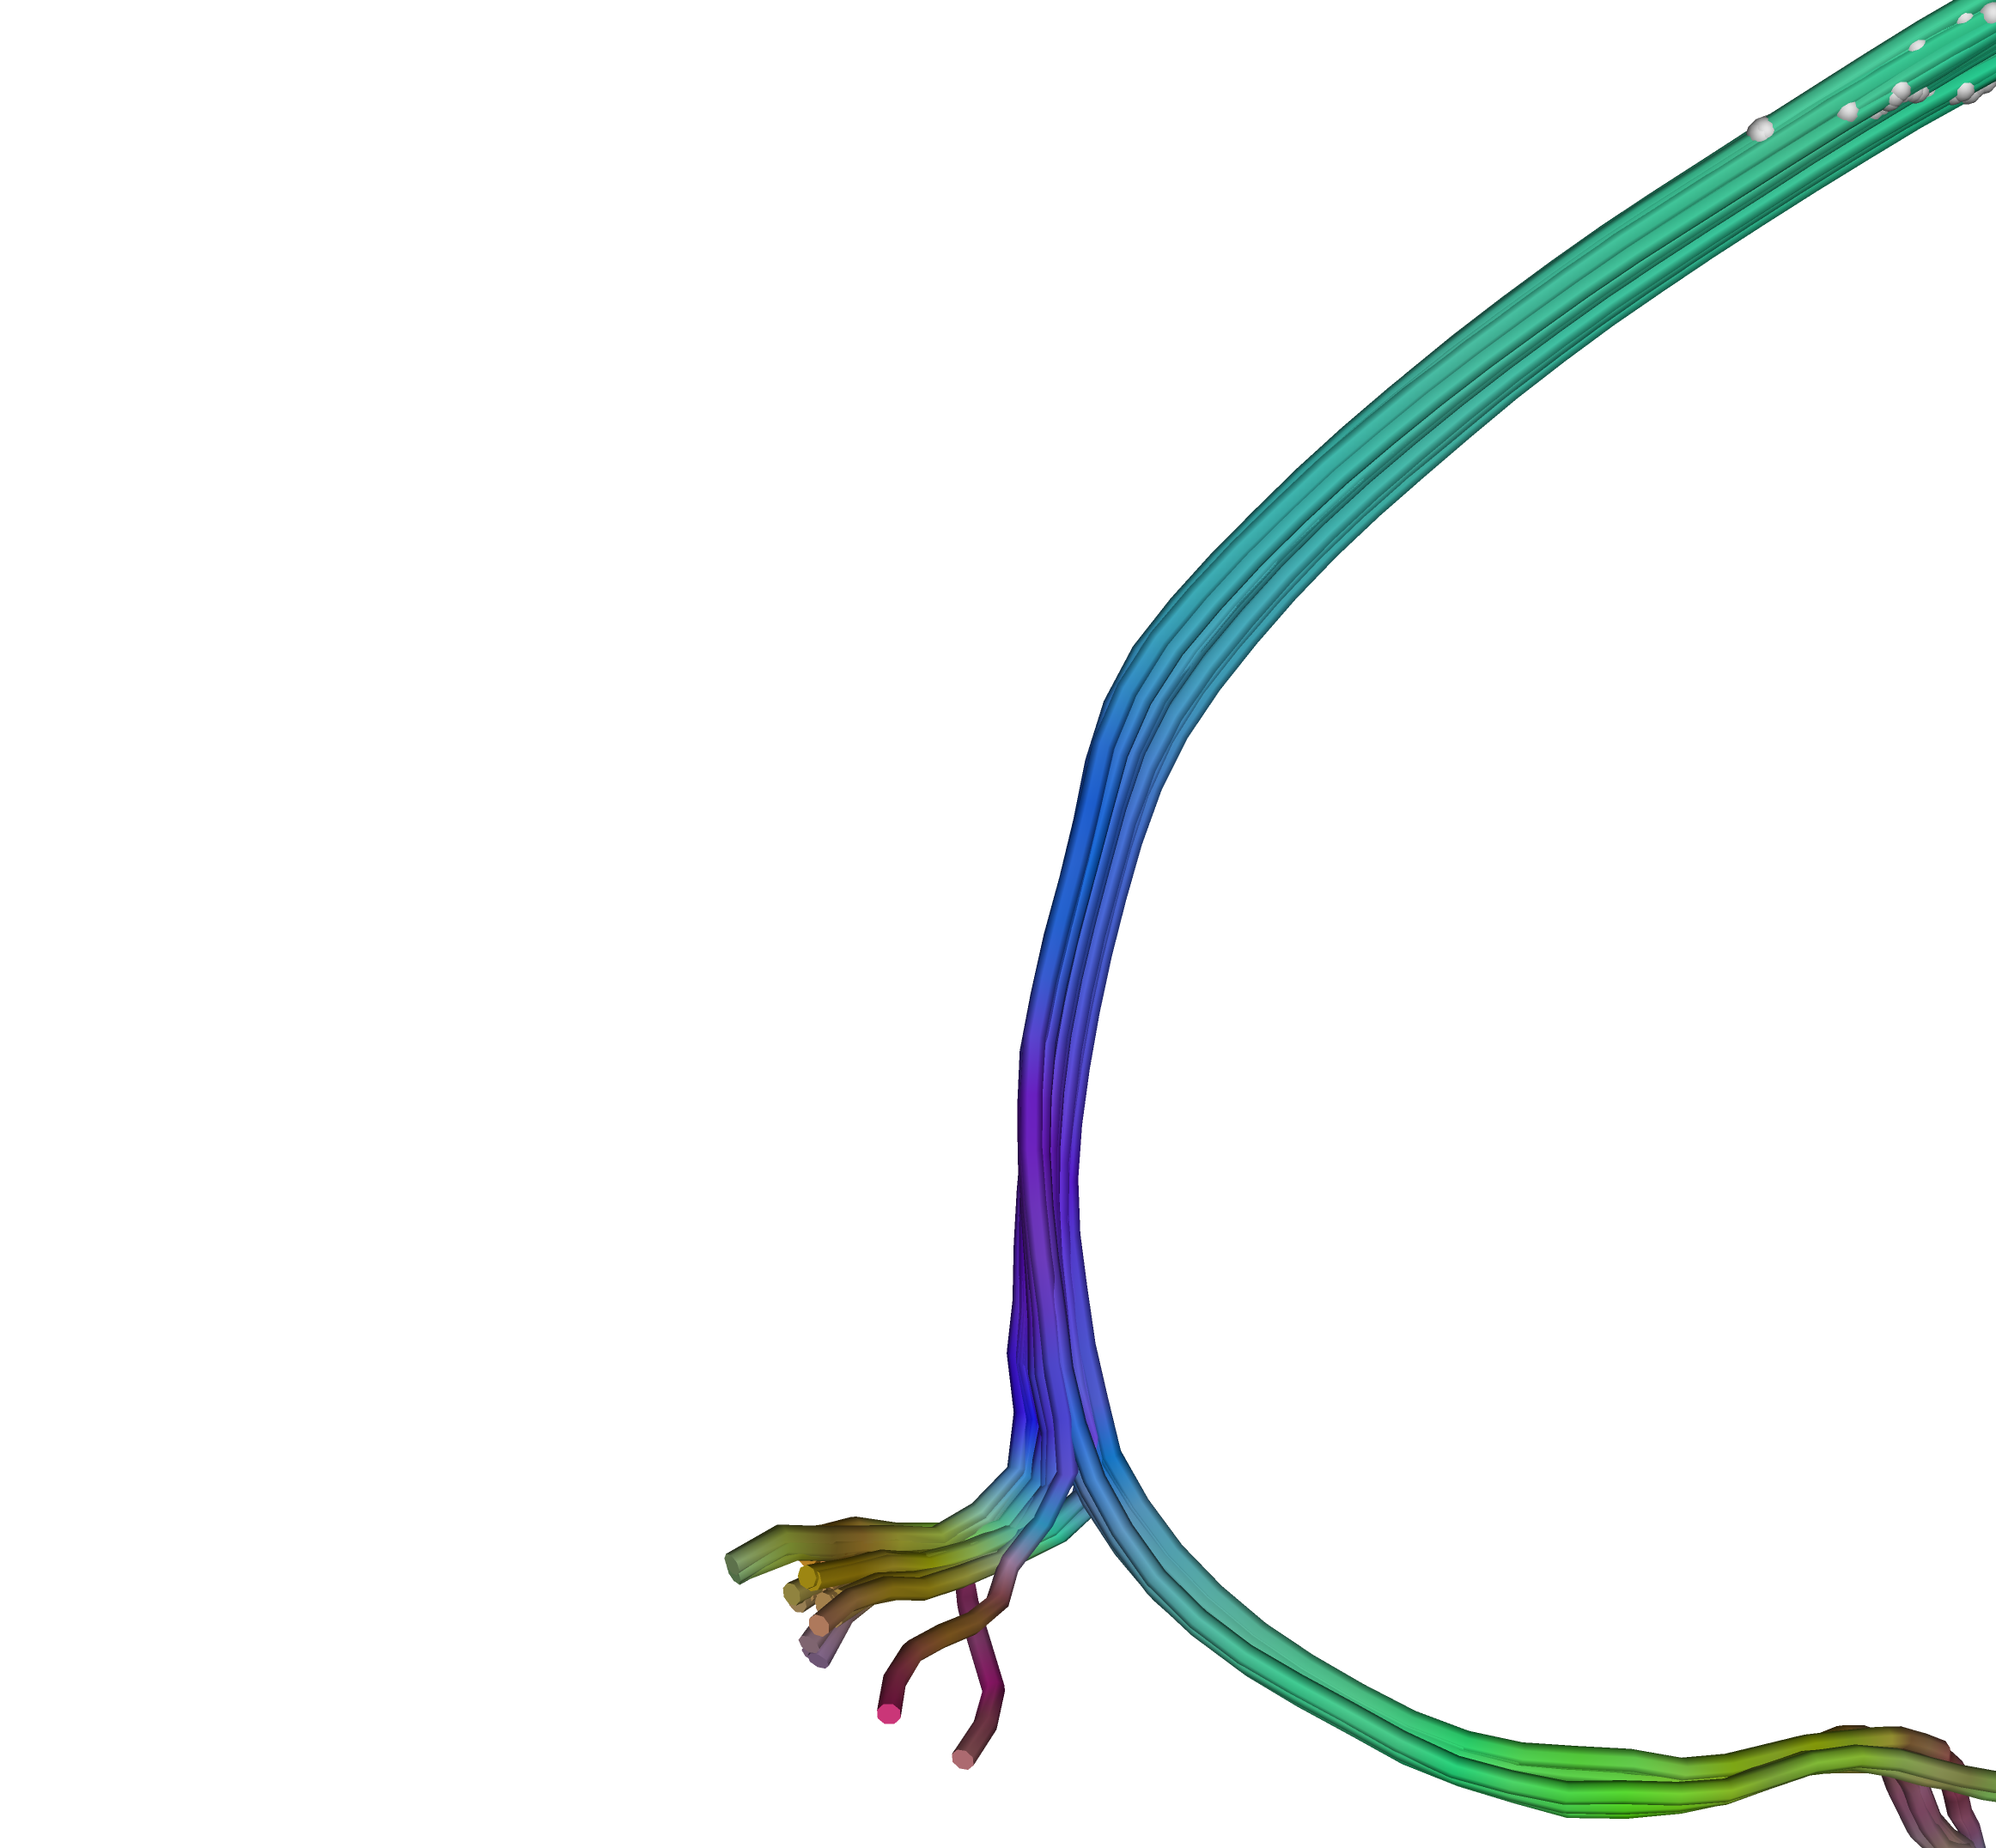
\includegraphics[width=\linewidth]{Trilinear}
% 		\caption{Trilinear interpolation}
% 	\end{subfigure}
% 	\caption{Comparison of nearest neighbor interpolation and trilinear
% 	interpolation in the anterior part of the cingulum. Seed points are marked
% 	by the white dots in the upper right corner. The trilinear interpolation
%         is superior with respect to following the tract curvature, and remaining within the correct tract.}

% 	\label{fig:interpolation-comparison}
% \end{figure}

% Our previous work \cite{Gruen:2021} avoided the complications from having to find such matchings by simply using nearest neighbor interpolation. Fig.~\ref{fig:interpolation-comparison} illustrates that trilinear interpolation permits a more accurate reconstruction of curved tracts, in this example, the anterior part of the cingulum. Starting from seeds (grey spheres) on the upper right, it is obvious that trilinear interpolation~(b) permits a larger number of streamlines to successfully track through the strongly curved part of the cingulum. Moreover, with nearest neighbor interpolation, some streamlines get diverted into the forceps minor of the corpus callosum.

%Further, the local optimal
%configuration is cached. Using this, we only have to calculate the assignments
%once for each voxel which we are tracking through and reduce the time
%consumption of trilinear interpolation dramatically. 
%To initialize the trilinear interpolation, we take the directions of the nearest voxel as group means.

% No need to repeat this?
%\begin{align}
%	\text{Sym} \left( r  \right) & \rightarrow \mathbb{R}_+ \\ 
%	Z & \mapsto \sum \| \sgn \left( \langle \mathbf{v}_{Z \left( i \right)}
%	, \bar{\mathbf{v}}_i \rangle  \right) \mathbf{v}_{Z \left( i \right)} -
%\bar{\mathbf{v}}_i
%	\|
%\end{align}
% We only update the group means if a group mean is not defined.
%Then we solve the above minimization problem for each vertices and assign the direction as new
%group mean. Afterwards, we rerun the minimization for all vertices to get a
%close approximation of the optimal configuration. This is done,
%to reduce the time consumption drastically. 

Given the interpolated directions $\mathbf{v}_i$ at the current point, we
reorient them to have a non-negative inner product with the current tracking
direction $\mathbf{w}$. We select one of the $r$ possible directions by assigning each unit direction $\mathbf{v}_i$ with volume fraction
$\lambda_i$ for $i \in \left\{ 1 , \dots , r \right\}$ a probability following the probability
scheme
\begin{equation}
  \label{eq:probabilistic-selection}
	p \left( \mathbf{v}_i \right) \coloneqq \frac{ \mathbb{1}_{\lbrace\theta_i <
		\frac{1}{4} \pi \rbrace} \lambda_i \cos \left( \left( \frac{9}{2\sqrt{2
\pi}} \theta_i \right)^2 \right)^2}{\sum_j \mathbb{1}_{\lbrace\theta_j <
		\frac{1}{4} \pi \rbrace} \lambda_j \cos \left( \left( \frac{9}{2\sqrt{2
\pi}} \theta_j \right)^2 \right)^2 },   
\end{equation}
where $\theta_i$ denotes the angle between the possible direction $\mathbf{v}_i$
and the current direction $\mathbf{w}$. \added{The indicator function $\mathbb{1}_{\lbrace\theta_i <\frac{1}{4} \pi \rbrace}$ restricts the maximum angle to $45$ degrees, to limit diversions into neighboring tracts.} We note that the use of trilinear interpolation allowed us to make this threshold slightly stricter compared to our prior work \cite{Gruen:2021}.
%
Equation~(\ref{eq:probabilistic-selection}) assigns almost the same probability to directions with angles below 20 degrees, which coincides with the limited angular resolution of
spherical deconvolution \cite{TOURNIER20071459}. 

This iterative algorithm proceeds until we either reach a region with an overall white matter volume fraction below $0.3$, or the summed angle over the last $30$ mm is greater than
$130$ degrees. This prevents streamlines from going back and forth. In the latter case,
the entire streamline gets removed. 

\subsection{Postprocessing}
\label{sec:postprocessing}
While diffusion MRI is able to reconstruct most major white
matter tracts, it is known to yield many false
positives, which have to be removed according to anatomical knowledge
\cite{MaierHein:2017}. %Further, the probabilistic tracking approach
%generates outliers with low density, which have to be removed to have a proper
%output. 

Therefore, we define inclusion and exclusion regions for each tract. If a streamline intersects with an exclusion region, or if it  does not intersect with all inclusion regions, the whole streamline is discarded. All regions
are set carefully for a reference subject according to the protocols in
\cite{Wakana:2007}.
The remaining subjects are linearly registered to the reference using FSL's \texttt{flirt} \cite{FSL}, and the transformation is used to transfer the regions automatically.

Moreover, we remove obvious outliers by creating a density map for each streamline
bundle. Therefore, we count the number of streamlines intersecting each voxel.
All streamlines are cut off at the first intersection with a low density
area starting from the seed. The density threshold is defined for the
reference subject and then mapped to all other subjects according to the ratio of seed points.

%%% Local Variables:
%%% mode: latex
%%% TeX-master: "../main"
%%% End:
